% LaTeX Article Template - customizing header and footer
\documentclass{article}

\newtheorem{thm}{Theorem}

% Set left margin - The default is 1 inch, so the following
% command sets a 1.25-inch left margin.
\setlength{\oddsidemargin}{0.25in}

% Set width of the text - What is left will be the right margin.
% In this case, right margin is 8.5in - 1.25in - 6in = 1.25in.
\setlength{\textwidth}{6in}

% Set top margin - The default is 1 inch, so the following
% command sets a 0.75-inch top margin.
\setlength{\topmargin}{-0.25in}

% Set height of the header
\setlength{\headheight}{0.1in}

% Set vertical distance between the header and the text
\setlength{\headsep}{0.2in}

% Set height of the text
\setlength{\textheight}{9in}

% Set vertical distance between the text and the
% bottom of footer
%\setlength{\footskip}{0.15in}

% Set the beginning of a LaTeX document
\usepackage{multirow}
\usepackage{xcolor,colortbl}
\usepackage{fullpage}
\usepackage{graphicx}
\usepackage{amsthm}
\usepackage{amssymb}
\usepackage{amssymb}
\usepackage{algpseudocode}
\usepackage{caption}
\usepackage{float}
\usepackage{subcaption}
\usepackage{fancyvrb}
\graphicspath{%
    {converted_graphics/}% inserted by PCTeX
    {/}% inserted by PCTeX
}

\definecolor{black}{rgb}{0,0,0}
%%%%%%%%%%%%%%%%%%%%%%%%%%%%%

\begin{document}\title{Graph Theory\\ Spring 2017\\ Math-M330}         % Enter your title between curly braces
\author{Steven Myers}        % Enter your name between curly braces
\date{\today}          % Enter your date or \today between curly braces
\maketitle


% Redefine "plain" pagestyle
\makeatother     % `@' is restored as a "non-letter" character

% Set to use the "plain" pagestyle
\pagestyle{plain}

\section*{Undirected and Directed Graphs}

\paragraph{}
Graphs are comprised of vertices and edges. An edge serves as a connection between two vertices. We can also say that if there is an edge between vertices, then there is a pathway to get from one vertex to the next. Some examples of where graphs are applicable are graphs forming relationships between locations. Some vertices under that example could be cities, and their edges would represent the roads or pathways that lead from one city to the next. There are two types of graphs: \textit{undirected} and \textit{directed}. A directed graph is one where edges have a direction. So, an edge from vertex $A$ to vertex $B$ means that there is a connection from $A$ to $B$, but not from $B$ to $A$. On the contrary, undirected graphs do not have direction, so an edge between two vertices is bidirectional. If we have an edge between two vertices $A$ and $B$, then there is a path from $A$ to $B$, and $B$ to $A$. If a vertex has an edge with its own vertex, this edge is called a \textit{cycle}. In this document, we are not going to consider graphs that contain cycles.

\paragraph{}
We can classify vertices as being odd or even based on its \textit{degree}. The degree of a vertex is the number of ingoing and outgoing edges of the vertex. Alternatively, we can talk about the in-degree of a vertex as the number of edges entering a vertex, and the out-degree of a vertex being the number of edges exiting a vertex. So, a vertex is \textit{even} if its degree is even, and \textit{odd} if its degree is odd.

\begin{figure}[H]
    \centering
    \begin{minipage}{.45\textwidth}
        \centering
        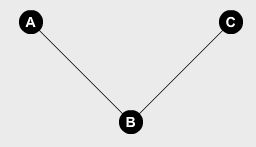
\includegraphics[width=.6\linewidth, height=.2\textheight]{undirected_graph}
        \caption{An undirected graph.}
    \end{minipage}
    \begin{minipage}{.45\textwidth}
        \centering
        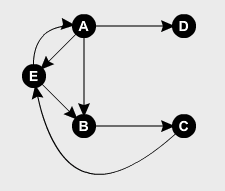
\includegraphics[width=.5\linewidth, height=.2\textheight]{directed_graph}
        \caption{A directed graph.}
    \end{minipage}
\end{figure}

\section*{Representing Graphs}
\paragraph{}
We can formally represent graphs as a collection of vertices and edges. A vertex is a singular point or constant, and an edge is tuple of two connected vertices. Two methods of concisely representing graphs in meaningful ways are \textit{adjacency matrices} and \textit{adjacency lists}. An adjacency matrix is a two dimensional array of boolean values. Its width and height are equal to the number of vertices in the graph, and every column and row represent a vertex. If the boolean value of some element at $(i,j)$ is true, then there is an edge from the vertex from row $i$ and a column $j$. This particular representation of a graph is useful only in undirected graphs, since there is no notion of direction. Adjacency matrices are symmetric, since the edges are undirected.\\\\

\begin{figure}[H]
\centering
\begin{subfigure}{.45\textwidth}
    \centering
    \begin{tabular}{|c|c|c|c|}
        \hline
         \cellcolor{black} & $A$ & $B$ & $C$\\
        \hline\hline
        $A$ & F & T & F\\
        \hline
        $B$ & T & F & T\\
        \hline
        $C$ & F & T & F\\
        \hline
    \end{tabular}
    \caption{An adjacency matrix for the graph in Figure 1.}
\end{subfigure}
\begin{subfigure}{.45\textwidth}
    \centering
    \begin{tabular}{|c||c|c|c|}
        \hline
        $A\rightarrow$ & $B$ & $D$ & $E$\\
        \hline
        $B\rightarrow$ & $C$ & & \\
        \hline
        $C\rightarrow$ & $E$ & &\\
        \hline
        $D\rightarrow$ & & &\\
        \hline
        $E\rightarrow$ & $A$ & $B$ &\\
        \hline
    \end{tabular}
    \caption{An adjacency list for the graph in Figure 2.}
\end{subfigure}
\end{figure}

\paragraph{}
Unlike adjacency matrices, an adjacency list is a convenient representation for directed graphs in addition to undirected graphs. It consists of a unique set of all of the vertices of the graph, and for each vertex there is a list or vector of the vertices that particular vertex shares an edge with.

\begin{figure}[H]
    \centering
    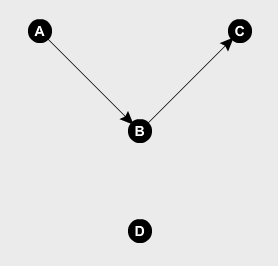
\includegraphics[width=.5\linewidth, height=.3\textheight]{disconnected_graph}
    \caption{A disconnected graph. Vertex $D$ is unreachable.}
\end{figure}

\section*{Euler Paths and Circuits}
\paragraph{}
A graph is \textit{traversable} if every vertex is reachable from any other vertex without reusing the same edge. To be traversable, a graph must be a \textit{connected} graph. A connected graph is one that has no unreachable vertices. Figure 4 shows a graph that is disconnected because vertex D cannot be reached by any other vertex. If a graph is traversable, then there is a sequence of edges to traverse the graph. This sequence of edges is called either an \textit{Euler circuit} or an \textit{Euler path}. An \textit{Euler path} is a path that uses every edge of a graph exactly once, and the path ends and begins on a \textbf{different} vertex. An \textit{Euler circuit} is also a path that uses every edge of a graph exactly once, but the path begins and ends on the \textbf{same} vertex.

\begin{figure}[H]
    \centering
    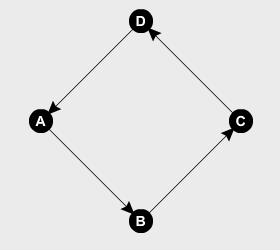
\includegraphics[width=.5\linewidth, height=.3\textheight]{euler_circuit}
    \caption{A graph with an Euler circuit.}
\end{figure}

\paragraph{}
Initially, we can attempt to find an Euler path given some graph $G$ by trying to find a way to explore all of the edges of $G$ without having to re-trace another edge. You can think of this as tracing a pencil over every edge in a graph without lifting the pencil up and without re-tracing over a previous edge. Looking back at Figure 2, if we start at any of the vertexes in the graph, it is impossible to find an Euler path. Every path we try to initiate, we will find that there is one vertex that we cannot visit without retracing a previous edge.

\paragraph{}
Figure 5 shows a graph that is connected, traversable, and has an Euler circuit. It doesn't matter what vertex we choose as a starting and ending point in this particular graph because all of the possible paths we can come up with happen to be Euler circuits. One particular Euler circuit would be the sequence of edges $\{(A,B),(B,C),(C,D),(D,A)\}$. An observation worthy of note is that all of the vertices in the graph for Figure 5 have a degree of 2. For every vertex, there is exactly one edge leaving the vertex and one edge entering the vertex.

\paragraph{}
For graphs that are particularly large, it would be impossbile to determine whether or not such a graph contained either an Euler circuit or path simply based on experimentation and brute force. It turns out there is a very simple way to determine whether or not some graph contains an Euler path or an Euler circuit. As mentioned above, all of the vertices in the graph for Figure 5 are \textit{even}, since their degree is two. We are guaranteed the fact that no matter what, there is some edge that will bring us to the same vertex again since there's exactly one edge leaving and entering every vertex.

\paragraph{}
\textit{Euler's Theorem}, hence the name \textit{Euler} circuits, tells us that for any connected graph $G$, $G$ contains an Euler circuit if and only if every vertex has even degree. We can prove this by induction. To prove this, we consider a trivial graph that contains an Euler circuit. Consider a graph $G$ with two vertices $A$ and $B$. If both vertices have a degree of two and there are no cycles, then the edges must be $\{(A,B), (B,A)\}$, which is and of itself an Euler circuit. This graph obviously contains an Euler circuit.

\paragraph{}
Now that we've successfully shown a trivial graph with vertices of even degree contains an Euler circuit, we can show by induction that an Euler circuit exists in a graph with more than 2 edges. If we have a graph $G$ with an arbritary number of vertices, but we know that the degree of every vertex is even, then we can choose any vertex $u$ and follow all un-visited edges at random. We know that we will eventually reach $u$ since every vertex we encounter also has an out-degree of at least one unused edge.

\paragraph{}
Now that we have shown the theorem for Euler circuits, we can discuss how to determine whether or not a graph contains an Euler path. Recall that an Euler path is a path through a graph that visits every edge exactly once, but begins and ends on different vertices. \textit{Euler's Theorem} states that a graph contains an Euler path if and only if a graph contains exactly two odd vertices.

\begin{figure}[H]
    \centering
    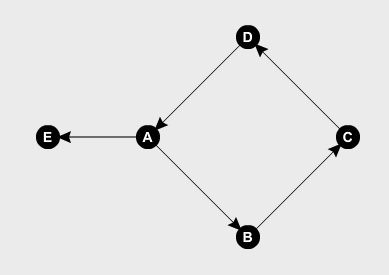
\includegraphics[width=.5\linewidth, height=.3\textheight]{euler_path}
    \caption{A graph with an Euler path. Vertices $A$ and $E$ are odd, while the rest are even.}
\end{figure}

\paragraph{}
To show that Euler's Theorem holds true for Euler paths, we can once again consider a trivial case in which there is a graph $G$ that has two odd vertices $A$ and $B$. $A$ has one edge with $B$, so both vertices have a degree of 1. An Euler path exists in the singleton set containing the edge $\{(A,B)\}$. So, Euler's Theorem holds for this trivial case.

\paragraph{}
If we consider a graph that has arbritarily many even vertices and exactly two odd vertices, then we can select one of the odd vertices that has an outdegree of at least one. Odd vertices have an even number of either incoming or outgoing edges. Therefore, there is always at least two outgoing edges for every ingoing edge, \textit{or} at least two incoming edges for every odd vertex. This makes sense for Euler paths because there is going to be a starting vertex with an odd out-degree an end vertex with odd in-degree, so there must be some path such that we start at the starting vertex and leave the vertex without returning to it, and finish on the ending vertex without having an unvisited edge.

\end{document}
